%=========================================================================
% (c) Michal Bidlo, Bohuslav K�ena, 2008

%%%%%%%%%%%%%%%%%%%%%%%%%%%%%%%%%%%%%%%%%%%%%%%%%%%%%%%%%%%%%%%%%%%%%%%%%%%%%%%%%%%%%%%%%%
\chapter{Introduction}





%%%%%%%%%%%%%%%%%%%%%%%%%%%%%%%%%%%%%%%%%%%%%%%%%%%%%%%%%%%%%%%%%%%%%%%%%%%%%%%%%%%%%%%%%%
\chapter{AES}
This chapter treats neccessary theoretical background of Advanced Encryption 
Standard, which is the default cipher, and as the text has been written the only
cipher, of Secure Real-time Transport Protocol used in VoIP communication.

\textit{Advanced Encryption Standard} is symetric block cipher which means 
it uses the same key for both encryption and decryption and encodes the
input in uniform sized blocks. The algorithm was developed to supersede
\textit{Data Encryption Standard} due to various security reasons\footnote
{ For instance COPACOBANA is FPGA based machine that could find 
an exhaustive key for DES in no longer than a week\cite{copacobana}.} in 
electronic data transmission. 

For this purpose National Institute of Standards and Technology (NIST)
announced public competition for new encryption standard in 1997 and 
considering multiple requirements the \textit{Rijndael}\footnote{ Rijndael
was original name of the AES as abreviation of authors' names -- Joan 
Daemen and Vincent Rijmen.} was selected as the most suitable algorithm
for the task\cite{AES-FIPS}. 

\section{Mathematical Preliminaries}
All the bytes in AES are interpreted as 8-bit values in finite field $2^8$.
For better readability the values are printed using hexadecimal notation.
Following mathematical therms and operations are used in AES aglorithm:

\subsubsection*{Galois field}
In algebra Galois field is finite field with finite number of elements.
Common notation is $GF(p^k)$ where $p$ is prime number and $k$ is positive
natural number. Therefore it is possible to classify the Galois fields 
by their size, because only single $GF(p^k)$ exists for each $p$ and $k$.
Characteristics of the field is equal to the $p$.

Each byte is in fact a polynomial with degree equal to 7 with coeficients
$b_i$ 0 or 1 and this notation $b_7x^7 + b_6x^6 + b_5x^5 + b_4x^4 + b_3x^3
+ b_2x^2 + b_1x^1 + b_0$. The decimal number 95 could be represented as:
\begin{itemize}
\item $5F$ in hexadecimal
\item $0101~1111$ in binary as a byte
\item $x^6 + x^4 + x^3 + x^2 + x^1 + 1$ as polynomial with degree equal to 7
\end{itemize}

\subsubsection*{Addition}
Addition is defined as addition of coeficinets of both polynomials modulo
2. This operation has the same result as bitwise XOR and because 
each value is its own inversion, addition and substraction are equal
operations.

\subsubsection*{Multiplication}
Multiplication is defined as multiplication of both polynomials modulo
irreducible polynomial of degree eight. For AES the irreducible polynom
is defined as
\begin{equation}
m(x) = x^8 + x^4 + x^3 + x + 1
\end{equation}

\subsubsection*{Multiplication by $x$}
Multiplication of binary polynomial by polynomial $x$ results in polynomial of
higher degree therefore the result must be reduced modulo $m(x)$. Following
equation is the binary polynomial multiplied by polynomial $x$.

\begin{equation}
b_7x^8+b_6x^7+b_5x^6+b_4x^5+b_3x^4+b_2x^3+b_1x^2+b_0x
\end{equation} 

If $b_7 = 1$ the result must be XORed with the polynomial $m(x)$. This operation
can be accomplished as bitwise left shift and XOR with $1B$.

\section{Algorithm Description}
The AES is block cipher, therefore both encryption and decryption processes
are performed on a matrix of 4x4 bytes called \textit{state}. Even though
state has fixed block size 128-bit, supported key sizes are 128-bit, 196-bit
and 256-bit. 

Encryption process as described in pseudocode \ref{encr} has 4 operations 
perfomed on each state of the data in specific number of cycles which 
varies from key length.
\begin{itemize}
\item 10 cycles for 128-bit key
\item 12 cycles for 196-bit key
\item 14 cycles for 256-bit key
\end{itemize}

\begin{algorithm}
\caption{AES encryption}
\label{encr}
\begin{algorithmic}
\State \textbf{Cipher(State, Key)}
\State state $\gets AddRoundKey($State, Key[0]$)$
\vspace{0.5em}
\For{$i \gets (1..n-1)$}
    \State state $\gets SubBytes($state$)$
    \State state $\gets ShiftRows($state$)$
    \State state $\gets MixColumns($state$)$
    \State state $\gets AddRoundKey($state, Key[i]$)$
\EndFor
\vspace{0.5em}
\State state $\gets SubBytes($state$)$
\State state $\gets ShiftRows($state$)$
\State state $\gets AddRoundKey($state, Key[n]$)$
\vspace{0.5em}
\State $return$ state
\end{algorithmic}
\end{algorithm}

\subsubsection*{Key Expansion}
Round keys are derived from cipher key through process called \textit{key 
expansion}. For the ciphering and deciphering purposes, the round keys could be 
thought as array of 4x4 8-bit values, which length is 10, 12 or 14 according to 
the used key size. The first matrix is copy of first 128 bits of cipher key. The
following round keys are always calculated from the previous key and 
\textit{rcon} array as explained in the algorithm \ref{keyexp}.

\begin{algorithm}[H]
\caption{Key Expansion}
\label{keyexp}
\begin{algorithmic}
\State \textbf{ExpandRoundKey(Key, size)}
\State rk[0] $\gets$ Key[0]
\vspace{0.5em}
\For {$i \gets (1..size)$}
    \State k.col(0) $\gets$ Key[$i-1$].col(3).rotate(1).map(sbox 
	    $\oplus$ Key[$i-1$].col(0)) $\oplus$ rcon
    \For {$j \gets (1..3)$}
        \State k.col($j$) $\gets$ Key[$i$-1].col($j$) $\oplus$ k.col($j-1$)
    \EndFor
    \State rk[$i$] $\gets$ k
\EndFor
\vspace{0.5em}
\State $return$ rk
\end{algorithmic}
\end{algorithm}


\subsubsection*{Ciphering Process}
\texttt{AddRoundKey} is XOR operation on the state with specific round key. 
Round key is extracted from the cipher key in \textit{ExpandRoundKey}. Since
this operation uses XOR, it is its own inverse form as well.

\begin{table}[H]
\label{shift}
\begin{center}
\begin{tabular}{|c|c|c|c|}\hline%
 $s_{00}$ & $s_{01}$ & $s_{02}$ & $s_{03}$  \\\hline
 $s_{10}$ & $s_{11}$ & $s_{12}$ & $s_{13}$  \\\hline
 $s_{20}$ & $s_{21}$ & $s_{22}$ & $s_{23}$  \\\hline
 $s_{30}$ & $s_{31}$ & $s_{32}$ & $s_{33}$  \\\hline
\end{tabular}
$\oplus$
\begin{tabular}{|c|c|c|c|}\hline%
 $k_{00}$ & $k_{01}$ & $k_{02}$ & $k_{03}$  \\\hline
 $k_{11}$ & $k_{12}$ & $k_{13}$ & $k_{10}$  \\\hline
 $k_{22}$ & $k_{23}$ & $k_{20}$ & $k_{21}$  \\\hline
 $k_{33}$ & $k_{30}$ & $k_{31}$ & $k_{32}$  \\\hline
\end{tabular}
$=$
\begin{tabular}{|c|c|c|c|}\hline%
 $a_{00}$ & $a_{01}$ & $a_{02}$ & $a_{03}$  \\\hline
 $a_{11}$ & $a_{12}$ & $a_{13}$ & $a_{10}$  \\\hline
 $a_{22}$ & $a_{23}$ & $a_{20}$ & $a_{21}$  \\\hline
 $a_{33}$ & $a_{30}$ & $a_{31}$ & $a_{32}$  \\\hline
\end{tabular}
\end{center}
\caption{AddRoundKey on state $s$ with key $k$ where $a_{ij} = s_{ij}\oplus k_{ij}$.}
\end{table}



\hspace{-1.5em}\texttt{ShiftRows} is performed on each row of the state matrix.
The first row is not shifted, second row is shifted by one byte to the left, 
third row is shifted by two bytes to the left and fourth row is shifted by three
bytes to the left. Inverted ShiftRows for decryption is simply reversion.

\begin{table}[H]
\label{shift}
\begin{center}
\begin{tabular}{|c|c|c|c|}\hline%
 $a_{00}$ & $a_{01}$ & $a_{02}$ & $a_{03}$  \\\hline
 $a_{10}$ & $a_{11}$ & $a_{12}$ & $a_{13}$  \\\hline
 $a_{20}$ & $a_{21}$ & $a_{22}$ & $a_{23}$  \\\hline
 $a_{30}$ & $a_{31}$ & $a_{32}$ & $a_{33}$  \\\hline
\end{tabular}
$\longrightarrow$
\begin{tabular}{|c|c|c|c|}\hline%
 $a_{00}$ & $a_{01}$ & $a_{02}$ & $a_{03}$  \\\hline
 $a_{11}$ & $a_{12}$ & $a_{13}$ & $a_{10}$  \\\hline
 $a_{22}$ & $a_{23}$ & $a_{20}$ & $a_{21}$  \\\hline
 $a_{33}$ & $a_{30}$ & $a_{31}$ & $a_{32}$  \\\hline
\end{tabular}
\end{center}
\caption{State on the right is the first state after ShiftRows is performed.}
\end{table}

\hspace{-1.5em}\texttt{MixColumns} together with ShiftRows provides diffusion in
the AES algorithm. During this operation each column of the state is multiplied 
in Galois field $2^8$ by matrix \ref{mix}.

\begin{equation}
\label{mix}
\left(
\begin{array}{cccc}%
 2 & 3 & 1 & 1  \\
 1 & 2 & 3 & 1  \\
 1 & 1 & 2 & 3  \\
 3 & 1 & 1 & 2  \\
\end{array}
\right)
\end{equation}

As a result of this multiplication, each column $[s_{0c}, s_{1c}, s_{2c}, 
s_{3c}]$ is replaced by the column $[a_{0c}, a_{1c}, a_{2c}, a_{3c}]$ which could 
be calculated:

\begin{equation}
\begin{array}{lllllllll}
a_{0c} &=& 2\cdot s_{0c} &\oplus& 3\cdot s_{3c} &\oplus& s_{2c} &\oplus& s_{1c} \\
a_{1c} &=& s_{1c} &\oplus& 2\cdot s_{0c} &\oplus& 3\cdot s_{3c} &\oplus& s_{2c} \\
a_{2c} &=& s_{2c} &\oplus& s_{1c} &\oplus& 2\cdot s_{0c} &\oplus& 3\cdot s_{3c} \\
a_{3c} &=& 3\cdot s_{3c} &\oplus& 2\cdot s_{2c} &\oplus& s_{1c} &\oplus& s_{0c}
\end{array}
\end{equation}


\hspace{-1.5em}\texttt{SubBytes} is non-linear transformation of the input 
\textit{state}. Each byte in the state matrix is replaced with byte from 
substitution array of 256 8-bit values called S-box. The S-box \ref{sbox} for 
encryption is generated by determining the multiplicative inverse for a given 
number in $GF(2^8)$ Rijndael's finite field and then affine transformation. 
The S-box \ref{invsbox} for decryption uses the same matrix but has first 
applied addine transformation and then the multiplicative
inverse. For implementation purposes both S-boxes are precomputed. 


\begin{equation}
\label{sboxdef}
  \left[\begin{array}{c}
    y_0\\
    y_1\\
    y_2\\
    y_3\\
    y_4\\
    y_5\\
    y_6\\
    y_7\\
  \end{array}\right]
  =
  \left[\begin{array}{cccccccc}
    1 & 0 & 0 & 0 & 1 & 1 & 1 & 1\\
    1 & 1 & 0 & 0 & 0 & 1 & 1 & 1\\
    1 & 1 & 1 & 0 & 0 & 0 & 1 & 1\\
    1 & 1 & 1 & 1 & 0 & 0 & 0 & 1\\
    1 & 1 & 1 & 1 & 1 & 0 & 0 & 0\\
    0 & 1 & 1 & 1 & 1 & 1 & 0 & 0\\
    0 & 0 & 1 & 1 & 1 & 1 & 1 & 0\\
    0 & 0 & 0 & 1 & 1 & 1 & 1 & 1\\
  \end{array}\right]
  \left[\begin{array}{c}
    x_0\\
    x_1\\
    x_2\\
    x_3\\
    x_4\\
    x_5\\
    x_6\\
    x_7\\
  \end{array}\right]
  \oplus
  \left[\begin{array}{c}
    1\\
    1\\
    0\\
    0\\
    0\\
    1\\
    1\\
    0\\
  \end{array}\right]
\end{equation}

In this transformation $[x_0, .., x_7]$ is the multiplicative inverse as vector,
and $\oplus$ is XOR operation.

\begin{table}[H]
\label{sbox}
\begin{center}
\begin{tabular}{|c|cccccccccccccccc|}\hline%
      &  0 &  1 &  2 &  3 &  4 &  5 &  6 &  7 &  8 &  9 &  a &  b &  c &  d &  e &  f \\\hline
   00 & 63 & 7c & 77 & 7b & f2 & 6b & 6f & c5 & 30 & 01 & 67 & 2b & fe & d7 & ab & 76 \\ 
   10 & ca & 82 & c9 & 7d & fa & 59 & 47 & f0 & ad & d4 & a2 & af & 9c & a4 & 72 & c0 \\ 
   20 & b7 & fd & 93 & 26 & 36 & 3f & f7 & cc & 34 & a5 & e5 & f1 & 71 & d8 & 31 & 15 \\ 
   30 & 04 & c7 & 23 & c3 & 18 & 96 & 05 & 9a & 07 & 12 & 80 & e2 & eb & 27 & b2 & 75 \\ 
   40 & 09 & 83 & 2c & 1a & 1b & 6e & 5a & a0 & 52 & 3b & d6 & b3 & 29 & e3 & 2f & 84 \\ 
   50 & 53 & d1 & 00 & ed & 20 & fc & b1 & 5b & 6a & cb & be & 39 & 4a & 4c & 58 & cf \\ 
   60 & d0 & ef & aa & fb & 43 & 4d & 33 & 85 & 45 & f9 & 02 & 7f & 50 & 3c & 9f & a8 \\ 
   70 & 51 & a3 & 40 & 8f & 92 & 9d & 38 & f5 & bc & b6 & da & 21 & 10 & ff & f3 & d2 \\ 
   80 & cd & 0c & 13 & ec & 5f & 97 & 44 & 17 & c4 & a7 & 7e & 3d & 64 & 5d & 19 & 73 \\ 
   90 & 60 & 81 & 4f & dc & 22 & 2a & 90 & 88 & 46 & ee & b8 & 14 & de & 5e & 0b & db \\ 
   a0 & e0 & 32 & 3a & 0a & 49 & 06 & 24 & 5c & c2 & d3 & ac & 62 & 91 & 95 & e4 & 79 \\ 
   b0 & e7 & c8 & 37 & 6d & 8d & d5 & 4e & a9 & 6c & 56 & f4 & ea & 65 & 7a & ae & 08 \\ 
   c0 & ba & 78 & 25 & 2e & 1c & a6 & b4 & c6 & e8 & dd & 74 & 1f & 4b & bd & 8b & 8a \\ 
   d0 & 70 & 3e & b5 & 66 & 48 & 03 & f6 & 0e & 61 & 35 & 57 & b9 & 86 & c1 & 1d & 9e \\ 
   e0 & e1 & f8 & 98 & 11 & 69 & d9 & 8e & 94 & 9b & 1e & 87 & e9 & ce & 55 & 28 & df \\ 
   f0 & 8c & a1 & 89 & 0d & bf & e6 & 42 & 68 & 41 & 99 & 2d & 0f & b0 & 54 & bb & 16 \\ 
\hline
\end{tabular}
\end{center}
\caption{S-box for SubBytes transformation in hexadecimal notation.}
\end{table}

\section{Block Cipher Modes}
During encyption the same key is applied repeatedly on the uniform lenght blocks
of data to whose the message is separated into. Large amount of ciphered data 
with the same encryption key might present security threat unless the ciphering
algorithm provides form of randomization the output value. Such procedure might
be achieved by additional input value.

There are many variations on block cipher to provide this confidentiality\cite{
blockciphers}, for AES algorithm the most often used are \textit{counter 
mode} and \textit{f8-mode}. Both algorithms keep standard high level of 
confusion of the AES algorithm and provides necessary diffusion\footnote{
\textit{Confusion} and \textit{diffusion} are basic two properties of secure 
cipher introduced by Claude Shannon\cite{shannon}.}.

Both algorithms share some similar terminology and acronyms:
\begin{itemize}
\item $IV$ -- initial value used for encrypting the first block
\item $C_i$ -- ciphertext block number $i$
\item $P_i$ -- plaintext block number $i$
\item $E_K$ -- encryption function
\item $D_K$ -- decryption function
\end{itemize}

\subsubsection*{Counter Mode}
The counter mode (CTR) turns AES block algorithm into stream cipher with 
possibility for parallel computations\cite{parallelctr}. It is possible to 
decrypt the cipher text even with loss of number of blocks because the encrypted
blocks are not dependent on the previous blocks. Instead the additional 
diffusion value are achieved by specific counter. 

Equation \ref{ctr1} describes computation of counter value, equation \ref{ctr2}
describes ciphering the counter value, equation \ref{ctr3} is encryption process
-- XOR operation of plaintext with encrypted counter value which produces 
ciphered text and equation \ref{ctr4} is decryption process.

\begin{eqnarray}
\label{ctr1}
CTR_i &=& (IV + i-1)\mod 2^B \\
\label{ctr2}
H_i &=& E_K(CTR_i, key) \\
\label{ctr3}
C_i &=& P_i \oplus H_i \\
\label{ctr4}
P_i &=& C_i \oplus H_i \\
\end{eqnarray} 

The last block of the plaintext doesn't have to be padded\footnote{ Padding 
can be used for the plaintext that is not alligned to the multiplies of the 
block.}, it is common to use only the most significant bits of ciphered counter
to be XORed with plaintext in cipher algorithm (and in similar way for
deciphering). 


\subsubsection*{F8-mode}
The f8-mode is a variant of commonly known Output Feedback Mode (OFB)
\cite{blockciphers} with more elaborate initialization and feedback function
\cite{rfc3711}. The first output block $O_1$ is computed from $IV$, then it
is XORed with plaintext to produce the first ciphertext block. The output block
from previous step $O_{j-1}$ is used to compute the current output block $O_j$
which is always XORed with current plaintext in encryption algorithm. 

The equation \ref{ofb0} describes the improved initializing function where
$m$ is the mask. The equations \ref{ofb1} and \ref{ofb2} describes computation 
of value, which is used for ciphering algorithm to produce output values in 
equation \ref{ofb3}. Equation \ref{ofb4} describes ciphering and equation 
\ref{ofb5} describes deciphering.

\begin{eqnarray}
\label{ofb0}
IV' &=& E_K(IV, key \oplus m)\\
\label{ofb1}
I_1 &=& IV' \\
\label{ofb2}
I_j &=& O_{j-1} \oplus IV' \oplus j \\
\label{ofb3}
O_j &=& E_K(I_j, key) \\
\label{ofb4}
C_j &=& P_j \oplus O_j \\
\label{ofb5}
P_j &=& C_j \oplus O_j
\label{}
\end{eqnarray}



%\begin{table}[H]
%\label{invsbox}
%\begin{center}
%\begin{tabular}{|c|cccccccccccccccc|}\hline%
%      &  0 &  1 &  2 &  3 &  4 &  5 &  6 &  7 &  8 &  9 &  a &  b &  c &  d &  e &  f \\\hline
%   00 & 63 & 7c & 77 & 7b & f2 & 6b & 6f & c5 & 30 & 01 & 67 & 2b & fe & d7 & ab & 76 \\ 
%   10 & ca & 82 & c9 & 7d & fa & 59 & 47 & f0 & ad & d4 & a2 & af & 9c & a4 & 72 & c0 \\ 
%   20 & b7 & fd & 93 & 26 & 36 & 3f & f7 & cc & 34 & a5 & e5 & f1 & 71 & d8 & 31 & 15 \\ 
%   30 & 04 & c7 & 23 & c3 & 18 & 96 & 05 & 9a & 07 & 12 & 80 & e2 & eb & 27 & b2 & 75 \\ 
%   40 & 09 & 83 & 2c & 1a & 1b & 6e & 5a & a0 & 52 & 3b & d6 & b3 & 29 & e3 & 2f & 84 \\ 
%   50 & 53 & d1 & 00 & ed & 20 & fc & b1 & 5b & 6a & cb & be & 39 & 4a & 4c & 58 & cf \\ 
%   60 & d0 & ef & aa & fb & 43 & 4d & 33 & 85 & 45 & f9 & 02 & 7f & 50 & 3c & 9f & a8 \\ 
%   70 & 51 & a3 & 40 & 8f & 92 & 9d & 38 & f5 & bc & b6 & da & 21 & 10 & ff & f3 & d2 \\ 
%   80 & cd & 0c & 13 & ec & 5f & 97 & 44 & 17 & c4 & a7 & 7e & 3d & 64 & 5d & 19 & 73 \\ 
%   90 & 60 & 81 & 4f & dc & 22 & 2a & 90 & 88 & 46 & ee & b8 & 14 & de & 5e & 0b & db \\ 
%   a0 & e0 & 32 & 3a & 0a & 49 & 06 & 24 & 5c & c2 & d3 & ac & 62 & 91 & 95 & e4 & 79 \\ 
%   b0 & e7 & c8 & 37 & 6d & 8d & d5 & 4e & a9 & 6c & 56 & f4 & ea & 65 & 7a & ae & 08 \\ 
%   c0 & ba & 78 & 25 & 2e & 1c & a6 & b4 & c6 & e8 & dd & 74 & 1f & 4b & bd & 8b & 8a \\ 
%   d0 & 70 & 3e & b5 & 66 & 48 & 03 & f6 & 0e & 61 & 35 & 57 & b9 & 86 & c1 & 1d & 9e \\ 
%   e0 & e1 & f8 & 98 & 11 & 69 & d9 & 8e & 94 & 9b & 1e & 87 & e9 & ce & 55 & 28 & df \\ 
%   f0 & 8c & a1 & 89 & 0d & bf & e6 & 42 & 68 & 41 & 99 & 2d & 0f & b0 & 54 & bb & 16 \\ 
%\hline
%\end{tabular}
%\end{center}
%\caption{Inverse S-box for SubBytes transformation in hexadecimal notation.}
%\end{table}





%\begin{algorithm}
%\caption{AES decryption}
%\label{decr}
%\begin{algorithmic}
%\State \textbf{Decipher(State, Key)}
%\State state $\gets AddRoundKey($State, Key[n]$)$
%\State state $\gets ShiftRows($state$)$
%\State state $\gets SubBytes($state$)$
%\vspace{0.5em}
%\For{$i \gets (n-1..1)$}
%    \State state $\gets AddRoundKey($state, Key[i]$)$
%    \State state $\gets MixColumns($state$)$
%    \State state $\gets ShiftRows($state$)$
%    \State state $\gets SubBytes($state$)$
%\EndFor
%\vspace{0.5em}
%\State state $\gets AddRoundKey($state, Key[0]$)$
%\vspace{0.5em}
%\State $return$ state
%\end{algorithmic}
%\end{algorithm}



%%%%%%%%%%%%%%%%%%%%%%%%%%%%%%%%%%%%%%%%%%%%%%%%%%%%%%%%%%%%%%%%%%%%%%%%%%%%%%%%%%%%%%%%%%
\chapter{Secure Real-time Transport Protocol}
To achieve confidentiality and neccessary security for real-time multimedia
transmission over TCP/IP connection there has been invented SRTP\cite{
rfc3711}. Except previously mentioned, it provides message
authentication and replay protection for both RTP and RTCP traffic, 
however, the thesis is going to focus on the implementation and computation
time of the security. The default cipher is AES in counter mode.

\section{Packet Structure}
SRTP packet can be described as RTP extension. It keeps the RTP fields of
the packet such as:
\begin{itemize}
\item Version (V) -- two bit number which currently is equal to 2.
\item Padding (P) -- boolean value whether the padding is set.
\item Extension (X) -- if this field is set, fixed header must be followed by
exactly one extension header.
\item CSRC count (CC) -- number of CSRC identifiers that follow the fixed header.
\item Marker (M) -- interpretation defined by a profile.
\item Payload Type (PT) -- identifies the type of payload
\item Sequence Number (SEQ) -- incremets by one for each RTP packet.
\item Timestamp (TS) -- reflecting the exact moment the payload was sampled.
\item Synchronization Source Identifier (SSRC) -- identifier of RTP synchronization 
source within the single RTP session.
\item Contributing Source Identifiers (CSRC) -- list of 0 to 15 items identifying
contributing sources.
\end{itemize}

The SRTP protocol defines that only payload is encrypted and also describes new 
fields in the RTP header.

\begin{itemize}
\item Master Key Identifier (MKI) -- unique identifier of the master key 
(previously signaled) to be used in session key derivation.
\item Authentication Tag -- carries message authentication data. If both
encryption and authentication are used, encryption should be applied first.
\end{itemize}

The packet length is variable and depends on number of CSRC used and length
of payload. The following scheme describes the packet with proportional
sizes of each field.

\begin{verbatim}
    0                   1                   2                   3
  0 1 2 3 4 5 6 7 8 9 0 1 2 3 4 5 6 7 8 9 0 1 2 3 4 5 6 7 8 9 0 1
  +-+-+-+-+-+-+-+-+-+-+-+-+-+-+-+-+-+-+-+-+-+-+-+-+-+-+-+-+-+-+-+-+<+
  |V=2|P|X|  CC   |M|     PT      |       sequence number         | |
  +-+-+-+-+-+-+-+-+-+-+-+-+-+-+-+-+-+-+-+-+-+-+-+-+-+-+-+-+-+-+-+-+ |
  |                           timestamp                           | |
  +-+-+-+-+-+-+-+-+-+-+-+-+-+-+-+-+-+-+-+-+-+-+-+-+-+-+-+-+-+-+-+-+ |
  |           synchronization source (SSRC) identifier            | |
  +=+=+=+=+=+=+=+=+=+=+=+=+=+=+=+=+=+=+=+=+=+=+=+=+=+=+=+=+=+=+=+=+ |
  |            contributing source (CSRC) identifiers             | |
  |                               ....                            | |
  +-+-+-+-+-+-+-+-+-+-+-+-+-+-+-+-+-+-+-+-+-+-+-+-+-+-+-+-+-+-+-+-+ |
  |                   RTP extension (OPTIONAL)                    | |
+>+-+-+-+-+-+-+-+-+-+-+-+-+-+-+-+-+-+-+-+-+-+-+-+-+-+-+-+-+-+-+-+-+ |
| |                          payload  ...                         | |
| |                               +-------------------------------+ |
| |                               | RTP padding   | RTP pad count | |
+>+-+-+-+-+-+-+-+-+-+-+-+-+-+-+-+-+-+-+-+-+-+-+-+-+-+-+-+-+-+-+-+-+<+
| ~                     SRTP MKI (OPTIONAL)                       ~ |
| +-+-+-+-+-+-+-+-+-+-+-+-+-+-+-+-+-+-+-+-+-+-+-+-+-+-+-+-+-+-+-+-+ |
| :                 authentication tag (RECOMMENDED)              : |
| +-+-+-+-+-+-+-+-+-+-+-+-+-+-+-+-+-+-+-+-+-+-+-+-+-+-+-+-+-+-+-+-+ |
|                                                                   |
+- Encrypted Portion*                      Authenticated Portion ---+
\end{verbatim}

\section{Cryptographic Context}
In order to implement SRTP stack in the application, it is necessary to
preserve certain information about each encrypted session, which is 
called \textit{cryptographic context}. It must consist of the following:

\begin{itemize}
\item Rollover Counter -- 32-bit unsigned number, records how many times 
has the RTP sequential number been reseted to zero passed the value 65~535.
\item Highest Received SEQ -- 16-bit unsigned number
\item Identifier of the Encryption Algorithm -- the cipher and its mode
\item Replay List -- containing indices of recently received and 
authenticated SRTP packets
\item MKI -- if the MKI is present in current session, the length
of the MKI field in octets, actual value of currently used MKI
\item Master Keys -- enumeration of random and secret master keys
and counter for each key of how many packets have been sent with
that key. Single Master Key identifies SRTP stream and corresponding SRTCP
stream.
\item Session Keys -- current key for encryption and authentication
including stored their lengths in \texttt{n\_e} and \texttt{n\_a}
\end{itemize}

And for every master key, the cryptographic context may contain also
random but possibly public \textit{Master Salt} which will be used in 
key derivation.

\section{Protocol Summary}
Main concers about the use of SRTP are whether the increase of computational
complexity and packet size don't make RTP hardly usable and what degree of
security does it provide.

\subsubsection*{Computational Overhead}
In VoIP communication the time has essential impact on the quality of
transmitted information, therefore it is important that ensuring the 
security of RTP wouldn't increase the latency over the acceptable level.
Among commont limitations of real-time communications 
belong\cite{perkins:rtp2003}:
\begin{itemize}
\item Maximal tolerable latency round-trip time 300ms.
\item Smaller packet loss than 5\%.
\item Sensitivity to factors that are difficult to objectively measure
such as jitter.
\end{itemize}



It has been proven that increase in size of the packet SRTP is
insignificant compared to the RTP\cite{srtp:analysis2, srtp:analysis1}.
Average throughput of secured VoIP is usually around 2\% more than 
unsecured VoIP.



\subsubsection*{Security}
VoIP suffers from many simillar security threats as other standard internet
services. 

\textit{Man in the middle} in computer security is form of active eavesdropping.
The attacker creates connections to both endpoints of the session which allows
him to monitor, record or modify the packets in communication making the 
endpoints believe that the conversation is secured. 
Protection against such attack could be achieved by key negotiating protocol
\textit{ZRTP} which is able to detect this activity\cite{rfc6189}.

\textit{Denial of service} is considered an attempt to make target machine unavailable
to to its intended users. Typical method of this attack is to saturate the target
machine with excessive requests that could lead to overloading the machine.
Replay protection mechanism of SRTP with replay lists and authentication headers
provide sufficient protection against DoS attack\cite{rfc3711}.



%%%%%%%%%%%%%%%%%%%%%%%%%%%%%%%%%%%%%%%%%%%%%%%%%%%%%%%%%%%%%%%%%%%%%%%%%%%%%%%%%%%%%%%%%%
\chapter{Parallel Programming Paradigm}
This chapter describes the basic ideas and techniques behind GPU parallel 
programming model and architecture. Following text will focus on possibilities
of efective implementation for GPGPU and integrated GPU in modern CPU using 
OpenCL framework, brief description of selected principles and development of
parallel applications. 

Parallel machines have impressive performance to cost ratio compared to the
common sequential machines\cite{Darlington93structuredparallel}, but bring well
known problems for software development such as run-time resource allocation
and resource sharing. Mapping parallel program to multiprocessor machine is
complex problem that needs to decide about task allocation, scheduling of
processes, communication patterns and much more.

\section{General Purpose GPU}
While current CPUs are powerfull and sofisticated chips, their design must be
focused on wide variety of tasks, therefore vast majority of resources might
not be as fully utilized as could have been. The GPU chips provide much better
theoretical performance for certain tasks for smaller price\cite{Owens:2007:ASO}.
Interest among developers has grown in using the power GPUs provide for other
tasks than graphics pipeline. 

In order to achieve improvement in certain algorithm it is neccessary to analyze
the procedures and find possibilities for parallelization and take under 
consideration that usage of additional processing unit brings computational 
overhead. The characteristics of such application are\cite{Owens:2008:GC}:

\begin{itemize}
\item Utilization of data-parallelism -- many non-graphical problems might be
separated into fractional procedures and computed separately, such as matrix 
calculations individially for each cell.
\item Large portion of computation -- GPU porcessors are optimized for 
computations over handling conditional evaluations.
\item Throughput over Latency -- computations on GPU are designed for large
overall throughput of entire data rather than short response time of each 
individual operation.
\end{itemize}

The current trend in development shows that parallel computations either in the
form of GPU computations and APU\footnote{ Accelerated Processing Unit -- 
in this context it means CPU with GPGPU chip.} are
worth examination and research. SIMD\footnote{ Single Instruction Multiple Data 
-- multiple processing elements that perform the same operation on multiple data 
points simultaneously\cite{Flynn:1972}.} has already proven it's value on 
improving performance with parallelization of various 
algorithms\cite{nvidia:sample, amd:apps}.

\subsubsection*{Architecture}

\{***Some smart text and picture of how GPU looks and works***\}





\subsubsection*{APU}
Usual solutions with graphics card can have high power consumption. The modern
trend and need of transportable forced development to reduce negative 
effects of GPUs while keeping as much of latest visual experience as 
possible\cite{apu:efficiency}.
Both solutions utilize a portion of computer's system RAM memory.

APU is Accelerated Processing Unit that is designed to accelerate certain
type of computations outside of CPU in single chip\cite{wiki:apu}. It could include 
GPU, FPGA or similar specialized processing unit. Among the best known there
are Intel HD Graphics\cite{intel:apu}, AMD Fusion\cite{amd:apu} and NVIDIA 
Project Denver\cite{nvidia:apu}.

\section{OpenCL}
Development for parallel computation brought need for infrastructure. OpenCL
is an industry standard framework fr programming heterogenous systems 
composed of a combination of CPUs, GPUs, DSP and other processing 
units\cite{opencl}. With OpenCL it is possible to write a software that will
run on wide variety of platforms from cell phones or computers to massive
supercomputers. 

The \textit{OpenCL programming language} has syntax based
on the language C with few additions and limitations arising from the design
and architecture of heterogenous platforms. Among most important limitations
it omits the use of recursion, function pointers and header files. On the 
other hand, the language is extended to the use of parallelism with build 
in types and synchronization. Also it defines many functions and four new
keywords as memory region qualifiers: \texttt{\_\_global}, 
\texttt{\_\_local}, \texttt{\_\_constant} and \texttt{\_\_private}.

For further reading of the text and better comprehensibility, there are
listed neccessary words from OpenCL terminology\cite{opencl}.
\begin{itemize}
\item Context -- contains one or more devices used for kernel execution
and are used for managing command queues, memory and program.
\item Kernel -- function written in OpenCL programming language that 
is executed on OpenCL device. 
\item Work-item -- instance of executing kernel. 
\item Work-group -- organisation of work-items. 
\item Command-queue -- interaction between the host and OpenCL
device through commands posted by the host and provides synchronization
methods for the execution of the commands.
\end{itemize}

OpenCL platform includes single \textit{host} that comunicates with the user
and the OpenCL program. The host is connected to one or more
OpenCL \textit{devices} where the \textit{kernels} are executed. 
\textit{Kernel} could be considered as the entry point between host and
GPU. In order to achieve parallelism, the device consists of many 
\textit{work-items} whose execute multiple instances of kernel at the same 
time. The work-items are organized in integer indexed orthogonal grid where 
the unique index of a work-item is called gloabl ID. The identification
of work-item is possible through combination of its local ID inside a specific
\textit{work-group} and the work-group global ID.

\subsubsection*{Platform Model}
The OpenCL provides a high-level abstraction model representing any heterogenous
platform. The \textit{host} is a bridge between parallel computations on one or
more devices and interaction with external environment. \textit{Device} could be
CPU, GPU, DSP or any other processing unit supporting OpenCL and consists
of compute units which are further divided into processing elements. 
\textit{Processing element} is abstraction of a work-item and \textit{compute unit} is 
in similar way representation of work-group.

\begin{figure}[H]
\centering
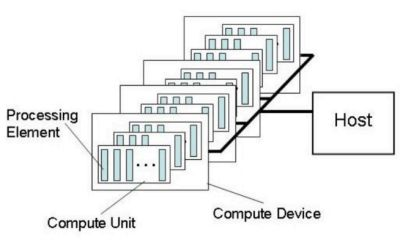
\includegraphics[width=10cm]{fig/opencl_platform_model.jpg}
\caption{OpenCL platform model with one host and multiple devices\cite{opencl}.}
\label{oclpm}
\end{figure}


\subsubsection*{Execution Model}
The OpenCL software executes on two levels
\begin{itemize}
\item \textbf{Host code} -- the OpenCL doesn't define any restrictions about the 
host part of the application, it defines only the interaction between host and devices.
It consists of selection and initialization of the context -- selected platform and 
devices.
\item \textbf{Device code} -- written in OpenCL programming language in the form of 
short functions, kernels, that usually transform an input array through series of 
processes into output array. It is compiled via OpenCL compiler and executed on the 
device's work-items.
\end{itemize}

The host program takes care of synchronization and plans the execution of each
kernel on the devices. Each instance of kernel runs in separate work-item and the
work-items within each work-group execute concurrently. 

\subsubsection*{Memory Model}
OpenCL defines two types of memory objects. The \textit{buffer object} is
versatile type that could be used for representation of any data type 
available in C or OpenCL language. The \textit{image object} is restricted 
to containing pictures only and is optimized for the specific needs of 
image processing.

OpenCL uses a hierarchicaly structured memory. The types differ in access time,
availability and types of usage\cite{opencl}:
\begin{itemize}
\item \textbf{Private Memory} -- each work-item has it's own private memory which 
could be thought of as analogy to CPU's registers. It is the fastest type of memory
used in OpenCL.
\item \textbf{Local Memory} -- designed for sharing data between work-items who 
belong to the same work group. It is used to reduce the number of accesses to the
global memory. Local memory is slower than private memory but faster than global
memory. The programmer is denied both direct access and control over local memory.
The analogy could be the cache in CPU.
\item \textbf{Global Memory} -- shared among all work-items in the same context.
\item \textbf{Host Memory} -- memory visible only for the host, OpenCL only defines
how the host interacts with OpenCL objects and constructs.
\end{itemize}

\hspace{-1.5em}
There could be another type of memory in graphic cards that OpenCL doesn't define

\begin{itemize}
\item \textbf{PCI Memory} -- type of memory that could be used by the program and
GPU, part of host memory. It is slower than global memory.
\end{itemize}



%%%%%%%%%%%%%%%%%%%%%%%%%%%%%%%%%%%%%%%%%%%%%%%%%%%%%%%%%%%%%%%%%%%%%%%%%%%%%%%%%%%%%%%%%%
\chapter{Implementation}
\cite{apu:crypto}




%%%%%%%%%%%%%%%%%%%%%%%%%%%%%%%%%%%%%%%%%%%%%%%%%%%%%%%%%%%%%%%%%%%%%%%%%%%%%%%%%%%%%%%%%%
\chapter{Testing}





%%%%%%%%%%%%%%%%%%%%%%%%%%%%%%%%%%%%%%%%%%%%%%%%%%%%%%%%%%%%%%%%%%%%%%%%%%%%%%%%%%%%%%%%%%
\chapter{Conclusion}


%=========================================================================
